\chapter{Ionization}

In this chapter the model, previously presented is modified to allow the ionization precesses. The main goal here is to find the ionization rate of a Majorana state, when the typical size of the photon is much smaller, than the gap int the spectrum.  Only regime with $ \abs{g_L}\ll g_R $ is considered --- even though the ionization for this condition is factorized, it contains it's own nontrivial physics with a number of different subregimes.

\section{Introducing the perturbation}

To study the ionization behavior of the system, it's necessary must modify the model considered in chapter \ref{chap:model}. It's reasonable to assume, that this perturbation will be present as an alternating voltage applied to the junction. This may alter the Hamiltonian (\ref{full_hamiltonian}) in two ways --- by the modification of the chemical potentials $ \mu_L, \mu_R $ and by making the superconducting phase difference $ \varphi=\phi_R-\phi_L $ time dependent. The second effect can be described by a Josephson relation:
\begin{gather}
	U\br{t}
	=
	\frac{\hbar}{2e}
	\frac{\partial\varphi\br{t}}{\partial t}
\end{gather}

The ionization voltage is assumed to be small compared to other energy parameters of the system, but this smallness is present in both effects. However, is the frequency $ \omega $ of the voltage is also small, the perturbation induced by the second effect will have additional big multiplier $ \frac{\Delta}{\omega} $ and will be much more important than the. In this chapter only this regime is taken under consideration.

The time dependence of phase difference is introduced as:
\begin{gather}
	\varphi\br{t}=\varphi_0+\alpha\cos\omega t
\end{gather}
where $ \varphi_0 $ is an initial time independent phase difference and $ \alpha $ is an amplitude of phase oscillations.

As was shown in section \ref{sec:elimintaing_longwave}, there exists a gauge transform $ U_\phi $, which may redistribute the phase difference between the wires, so the phase in a given wire can take any value. This ambiguity just reflects a  fact, that only phase difference $ \varphi $ is a observable quantity, but not the phases $ \phi_L $, $ \phi_R $ separately. However when treating the time dependent $ \phi\br{t} $, where the oscillating phase is present. Moreover, the voltage frequency $ \omega $ is assumed to be much smaller than not obly the superconducting gap $ \Delta $, but the spectrum gaps in both wires: $ \omega\ll g_R, \abs{g_L} $


The correct answer is that both left and right wires should get equal time-dependent phase with different signs: $ \phi_L=-\frac{\varphi_0}{2}-\frac{\alpha}{2}\cos \omega t $, $ \phi_R=\frac{\varphi_0}{2}+\frac{\alpha}{2}\cos \omega t $. Thus the superconducting terms in the wire Hamiltonians alter: $ \Delta_{\pm\frac{\varphi}{2}} \to\Delta_{\pm\frac{\varphi}{2}\pm \frac{\alpha}{2}\cos \omega t} $. Decomposing them in small $ \alpha $ one can explicitly write the perturbation and try to compute the ionization rate. However this way appears to be quite difficult as the overlaps of all the states 
present in both wires and at first it seems that the Majorana states has to much ways to ionize. To avoid this difficulty, the tunnel Hamiltonian approach is used.
\section{Tunnel Hamiltonian approach}
\label{sec:tunnel_hamiltonian}
The main idea of this method is to hide all the time dependence and the tunnel effect in one single operator. The local goal is to write the Hamiltonian as $ H=H_L+H_R+H_T $, where $ H_{L,R} $ are the Hamiltonians of the left and right wire without any contact (corresponding to zero tunneling: $ t=0 $), and $H_T  $ is a tunnel Hamiltonain both containing the time dependence and mixing the wavefunctions from different wires. 

Here the following notation is used.The Hamiltonians $ H_L $, $ H_R $ and $ H_T $ are 8x8 matrices in combined Nambu-Gorkov and LR-space. In LR-space they have the following form:
\begin{gather}
	H_L
	=
	\begin{pmatrix}
	h_L & 0 \\
	0 & 0
	\end{pmatrix}_{LR}
	\quad
	H_R
=
\begin{pmatrix}
0 & 0 \\
0 & h_R
\end{pmatrix}_{LR}
\quad
	H_T
=
\begin{pmatrix}
0 & h_T^\dagger \\
h_T & 0
\end{pmatrix}_{LR}	
\end{gather}
 The spinors with four components are corresponding to the unperturbed wavefunctions and are denoted as $ \big|\gamma_{0}\,\big> $,  for the Majorana state and $ \big|\varepsilon,L_{0}\,\big> $, $ \big|\varepsilon,R_{0}\,\big> $ for the contentious spectra in the left and in the right wires respectfully, and the corrections are denoted as $ \big|\gamma_{1}\,\big> $, $ \big|\varepsilon,L_{1}\,\big> $, $ \big|\varepsilon,R_{1}\,\big> $. These wavefunctions can be found in the appendix \ref{app:wavefunctions_with_corrections}.  In the the combined space of dimension 8 this spinors are:

\begin{gather}
	\Psi_{\gamma}=\begin{pmatrix}0\\
	\big|\gamma_{0}\,\big>
	\end{pmatrix}_{LR}+\begin{pmatrix}\big|\gamma_{1}\,\big>\\
	0
	\end{pmatrix}_{LR}+...\\\Psi_{R}=\begin{pmatrix}0\\
	\big|\varepsilon,R_{0}\,\big>
	\end{pmatrix}_{LR}+\begin{pmatrix}\big|\varepsilon,R_{1}\,\big>\\
	0
	\end{pmatrix}_{LR}+...\\\Psi_{L}=\begin{pmatrix}\big|\varepsilon,L_{0}\,\big>\\
	0
	\end{pmatrix}_{LR}+\begin{pmatrix}0\\
	\big|\varepsilon,L_{1}\,\big>
	\end{pmatrix}_{LR}+...
\end{gather}


The correct way to write $ H_T $ is to make it restoring the corrections from appendix \ref{app:wavefunctions_with_corrections}. To do so, one may write the unperturbed Green function of the system as:

\begin{multline}
	G_{0}\left(E\right)=\frac{1}{E+i0}\begin{pmatrix}0 & 0\\
	0 & \big|\gamma_{0}\,\big>\big<\gamma_{0}\,\big|
	\end{pmatrix}_{LR}+\int_{g_{L}}^{\infty}\frac{d\varepsilon}{N_{L}\left(\varepsilon\right)}\frac{1}{E+i0-\varepsilon}\begin{pmatrix}\big|\varepsilon,L_{0}\,\big>\big<\varepsilon,L_{0}\,\big| & 0\\
	0 & 0
	\end{pmatrix}_{LR}+\\+\int_{g_{l}}^{\infty}\frac{d\varepsilon}{N_{R}\left(\varepsilon\right)}\frac{1}{E+i0-\varepsilon}\begin{pmatrix}0 & 0\\
	0 & \big|\varepsilon,R_{0}\,\big>\big<\varepsilon,R_{0}\,\big|
	\end{pmatrix}_{LR}
\end{multline}
with $ N_{L,R} $ from (\ref{N_L_N_R_definition}). 
The corrections for the spinors should be calculated as:
\begin{gather}
	\Psi_{1}\left(E\right)=G_{0}\left(E\right)H_{T}\Psi_{0}\left(E\right)
\end{gather}
So, for the different states:
\begin{align}
	\big|\gamma_{1}\,\big>&=\int_{g_{L}}^{\infty}\frac{d\varepsilon}{N_{L}\left(\varepsilon\right)}\,\frac{1}{-\varepsilon+i0}\big|\varepsilon,L_{0}\,\big>\,\big<\varepsilon,L_{0}\,\big|h_{t}\big|\gamma_{0}\,\big>\\\big|E+i0,R_{1}\,\big>&=\int_{g_{L}}^{\infty}\frac{d\varepsilon}{N_{L}\left(\varepsilon\right)}\,\frac{1}{E-\varepsilon+i0}\big|\varepsilon,L_{0}\,\big>\,\big<\varepsilon,L_{0}\,\big|h_{t}\big|E\,R_{0}\big>
	\\
	\nonumber
	\big|E+i0,L_{1}\,\big>&=\frac{1}{E+i0}\big|\gamma_{0}\,\big>\,\big<\gamma_{0}\,\big|h_{t}^{\dagger}\big|E,L_{0}\,\big>+
	\\	
	&\qquad\qquad\qquad\qquad
	+\int_{g_{l}}^{\infty}\frac{d\varepsilon}{N_{R}\left(\varepsilon\right)}\,\frac{1}{E-\varepsilon+i0}\big|\varepsilon\,R_{0}\big>\,\big<\varepsilon,R_{0}\,\big|h_{t}^{\dagger}\big|E,L_{0}\,\big>
\end{align}

Now, multiplying the third equation by $ \big<\gamma_{0}\,\big| $ and $ \big<\epsilon,R_{0}\,\big |$, find:
\begin{gather}
	\big<\gamma_{0}\,\big|E+i0,L_{1}\,\big>=\frac{1}{E+i0}\,\big<\gamma_{0}\,\big|h_{t}^{\dagger}\big|E,L_{0}\,\big>\\\big<\epsilon,R_{0}\,\big|E+i0,L_{1}\,\big>=\frac{1}{E-\epsilon+i0}\big<\epsilon,R_{0}\,\big|h_{t}^{\dagger}\big|E,L_{0}\,\big>
\end{gather}
The l.h.s. of both equations above can be found explicitly with the help of appendix \ref{app:wavefunctions_with_corrections}. The result yields:
\begin{gather}
\label{tunnel_matrix_elements_maj-cont}
	\big<\gamma_{0}\,\big|h_{t}^{\dagger}\big|E,L_{0}\,\big>
	=
	4\sqrt{ug_{R}}
	\zeta^{2}t
	\left(e^{i\frac{\phi}{2}}+e^{-i\frac{\phi}{2}}\right)
	f\br{\frac{E}{\abs{g_L}}}
	\\
	\label{tunnel_matrix_elements_cont-cont}
	\big<\epsilon,R_{0}\,\big|h_{t}^{\dagger}\big|E,L_{0}\,\big>
	=
	-16u\zeta^{2}t
	\left(e^{i\frac{\phi}{2}}+e^{-i\frac{\phi}{2}}\right)
	f\br{\frac{E}{\abs{g_L}}}
	f\br{\frac{\varepsilon}{g_R}}
\end{gather}
where $ f\br{x}=\sqrt{x^2-1}\br{x+\sqrt{x^2-1}} $. The fact, that all energy dependences here are described by a single function $ f\br{x} $ insinuates that, maybe it's possible to make this calculations in a more beautiful way.

\section{Ionization rate for $ g_R\gg\abs{g_L} $}


\subsection{Time dependence of perturbation}

To obtain the ionization rate one should treat $ H_T $ as perturbation. For unperturbed system, described with $ H_0=H_R+H_L $ the electrons cannot get from wire to another, but $ H_T $ allows these processes, so the ionization can be described as a set of jumps from right to left wire (see fig. \ref{fig:tunneling})

\begin{figure}[H]
	\centering
	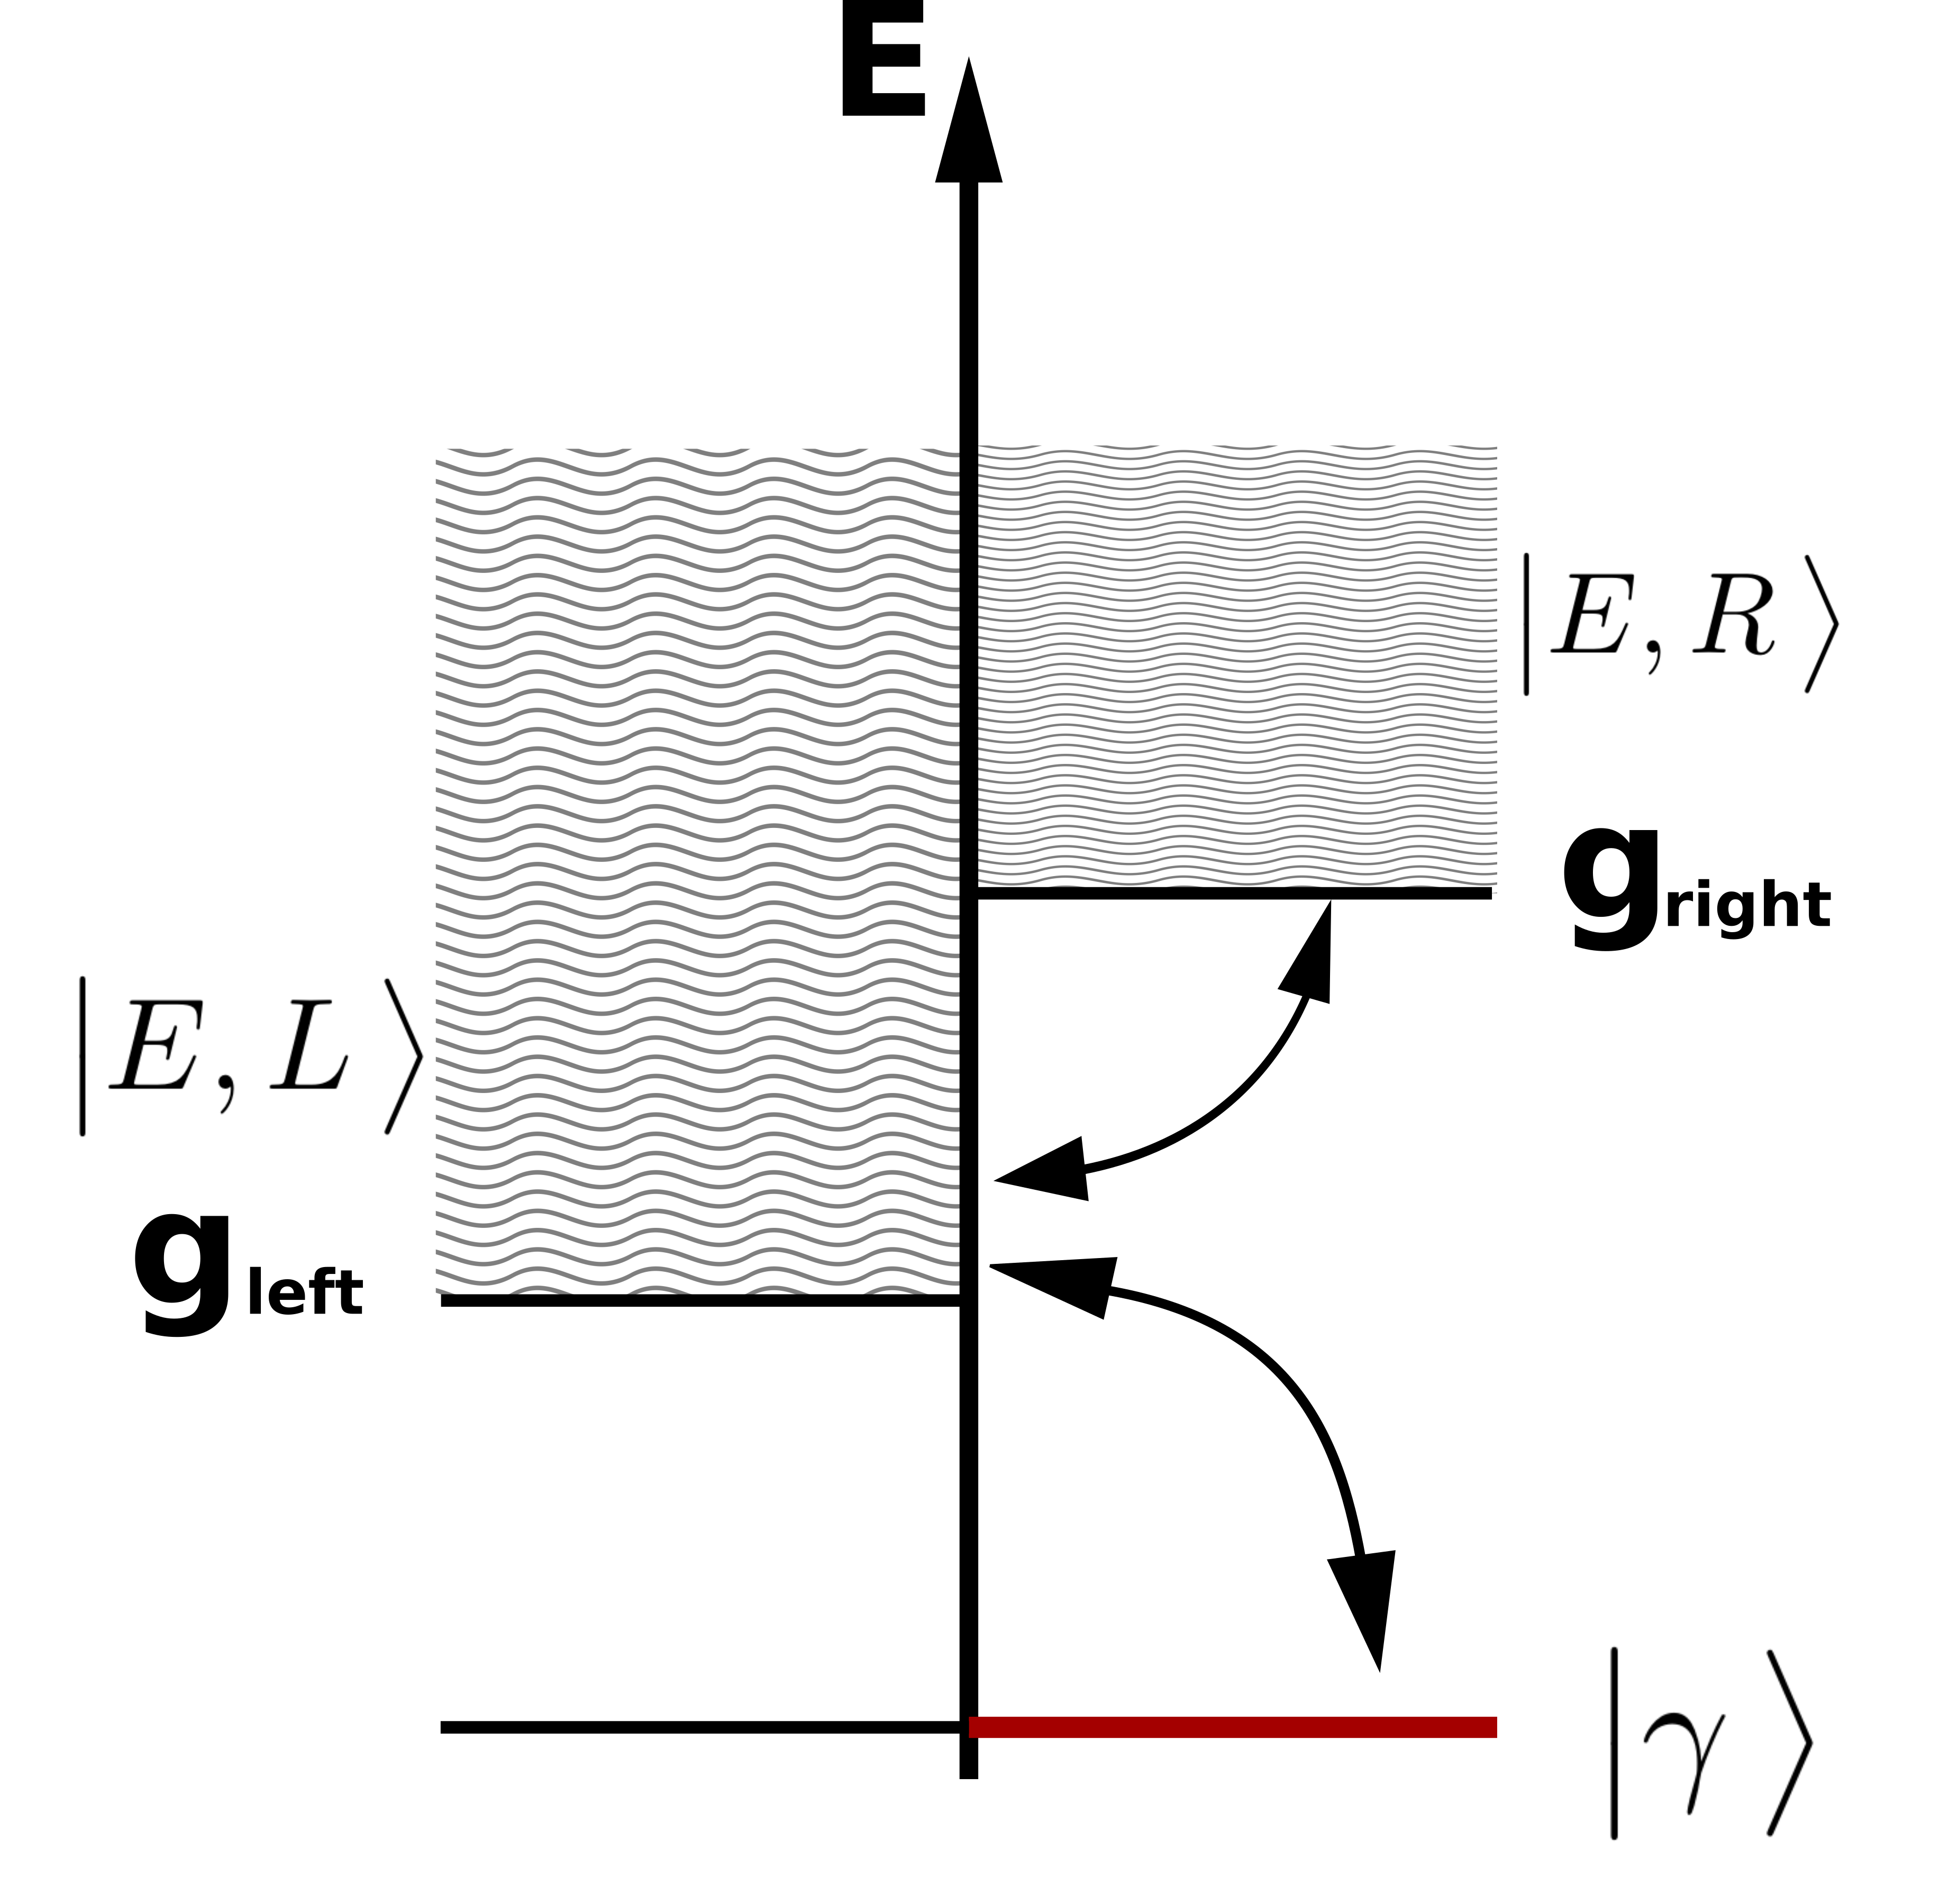
\includegraphics[width=0.6\linewidth]{images/tunneling}
	\caption{Ionization processes in terms of tunnel Hamiltonian}
	\label{fig:tunneling}
\end{figure}

The ionization rate can be calculated with the help of  (\ref{ionization_key}). To use this formula, one should decompose the  perturbation in Fourier series, as was done for (\ref{fourier_pertrubation}). From  (\ref{tunnel_matrix_elements_maj-cont}) one finds, that $ V=H_T\propto\cos\frac{\varphi\br{t}}{2} $ with $ \varphi=\phi_{0}+\alpha\cos\omega t $. Using $ \alpha\ll1 $ we write:
\begin{multline}
	e^{i\varphi/2}+e^{-i\varphi/2}\simeq e^{i\frac{\varphi_{0}}{2}}\sum_{n}\frac{(i\alpha/2)^{n}}{2^{n}n!}(e^{in\omega t}+e^{-in\omega t})+c.c=\\=\sum_{n}\frac{\alpha{}^{n}}{2^{2n}n!}(e^{in\omega t}+e^{-in\omega t})2\cos\left(\frac{\varphi_{0}}{2}+n\frac{\pi}{2}\right)
\end{multline}
so that $ V_{n}=V_{0}A_{n} $ with $ A_{n}=\frac{\alpha^{n}}{2^{2n-1}n!}\cos\left(\frac{\varphi_{0}}{2}+n\frac{\pi}{2}\right) $.

According to (\ref{tunnel_matrix_elements_maj-cont}) and (\ref{tunnel_matrix_elements_cont-cont}):
\begin{gather}
\label{tunnel_element_factorized}
	\langle\gamma|V_{0}|E\rangle=4\sqrt{ug_{R}}\zeta^{2}tf\br{\frac{E}{\abs{g_L}}}
\end{gather}

Here the focus is on the case where the topological gap is much larger than the trivial one. In this case, the right continuum has high energies and does not participate in the ionization process. Indeed,
\begin{gather}
	VG_{\epsilon}V=\frac{V|\gamma\rangle\langle\gamma|V}{\epsilon}+\intop_{|E_{R}|>g_{R}}\frac{V|E_{R}\rangle\langle E_{R}|V}{\epsilon-E_{R}}\frac{dE_{R}}{N_{R}(E_{R})}
\end{gather}
When $ g_{R}\gg\epsilon\sim g_{L} $, the second term can be neglected. Then, the product $ \dots V_{n}GV_{n'}GV_{n''}\dots $ factorizes into individual number-factors of the form $ \langle\gamma|V_{n}GV_{m}|\gamma\rangle $.

\subsection{Factorizing $ w_\mathcal{E} $}
Each entry in the sum within $ w_{\mathcal{E}} $ is a product of operators of the type $ \dots VGVGV\dots. $ In the limit we are now interested in, in the right wire only the Majorana mode is relevant. This means that the whole thing decomposes into a product of $ J_{nm}\equiv\langle\gamma|V_{n}|G_{E}|V_{m}|\gamma\rangle $, and the ionozation rate is proportional to:

\begin{gather}
	\mathcal{I}\propto
	\sum_N \sum_{\{n_i\}_M^N}\prod_{i=1}^{N}J_{n_in_{i+1}}
\end{gather}
Here the $ N $ has the meaning of total number of absorbed photons, $ M $ is the closet to $ \frac{\abs{g_L}}{\omega }$ integer, and the second sum is taken over all sets $ \{n_i\}_M^N $ such that there are $ N $ items in that set and $ \sum_i^N n_{i=1} = M$
 The $ n $,$ m $-dependence factors out so that $ J_{nm}=A_{n}A_{m}^{*}J_{0} $ where:

\begin{gather}
	J_{0}(E)=\langle\gamma|V_{0}G(E)V_{0}|\gamma\rangle\equiv\intop_{cont.}\frac{|\langle\gamma|V_{0}|\epsilon\rangle|^{2}}{E-\epsilon}\frac{d\epsilon}{N_L(\epsilon)}
\end{gather}

However on each ionization step  the particle can move a state with energy $ E $ or $ -E $. Taking this into account, one	 gets:

\begin{gather}
	J_{0}(E)
	=
	2E\intop_{|g_{L}|}^{\infty}\frac{|\langle\gamma|V_{0}|\epsilon\rangle|^{2}}{E^{2}-\epsilon^{2}}\frac{d\epsilon}{f(\epsilon)}
\end{gather}

recalling (\ref{tunnel_element_factorized}), obtain:
\begin{gather}
		J_{0}(E)
		=
		ET\frac{\left[-1+\sqrt{1-\lambda^{2}}\right]}{\lambda^{2}}
\end{gather}
where $ \lambda = \frac{E}{\abs{g_L}} $, $ T=\frac{g_R\br{\zeta^2t}^2}{\abs{g_L}} $.

Thus, the elementary block in our product becomes:
\begin{multline}
	\frac{J_{nm}}{E+n\omega}
	=
	A_{n}A_{m}\frac{J_{0}}{E+n\omega}\simeq A_{n}A_{m}T\frac{\left[-1+\sqrt{1-\lambda^{2}}\right]}{\lambda^{2}}
	=
	\\
	=\left(\frac{\alpha}{4}\right)^{n+m}B_{n}B_{m}^{*}T\frac{\left[-1+\sqrt{1-\lambda^{2}}\right]}{\lambda^{2}}
\end{multline}

where the parts that yield $ (\alpha/4)^{\mathcal{E}/\omega} $ for any trajectory and thus are factored out, as these parts do not affect summation and optimization. Thus one has $ B_{n}B_{m}T\frac{\left[-1+\sqrt{1-\lambda^{2}}\right]}{\lambda^{2}} $ to optimize.

Now consider a slice of the ionization process, i.e. a part of the full ionization product, which runs from energy $ E $ to $ E+\Delta E $ where $ \Delta E=M\omega $ with a large M. One can assume that within that process, a large number 2N of photons is absorbed, but energy does not change significantly, $ \Delta E\ll E $, so that $ \lambda $ can be considered a constant within that process. Denoting:
\begin{gather}
	T_{\lambda}=-4T\frac{\left[-1+\sqrt{1-\lambda^{2}}\right]}{\lambda^{2}}
\end{gather}

Then, one finds, that the ionization rate is $ \mathcal{I}\propto\mathcal{J} $ where:
\begin{gather}
\mathcal{J}=\sum_{\{n\}_{N}^{M}}\prod_{i=1}^{N}\frac{J_{n_{i}m_{i}}}{E}=\left(\frac{\alpha}{4}\right)^{M}\sum_{\{n\}_{2N}^{M}}(-T_{\lambda})^{\frac{N}{2}}\prod_{i=1}^{N}\frac{\cos(\frac{\varphi_{0}}{2}+\frac{\pi n_{2i}}{2})}{n_{2i}!}
\end{gather}
So to obtain the ionization rate up to a prexponential constant, one should compute $ \mathcal{J} $.